\documentclass[border=6pt]{standalone}
\usepackage{pgfplots}
\pgfplotsset{compat=1.18}
\usepgfplotslibrary{groupplots}
\begin{document}
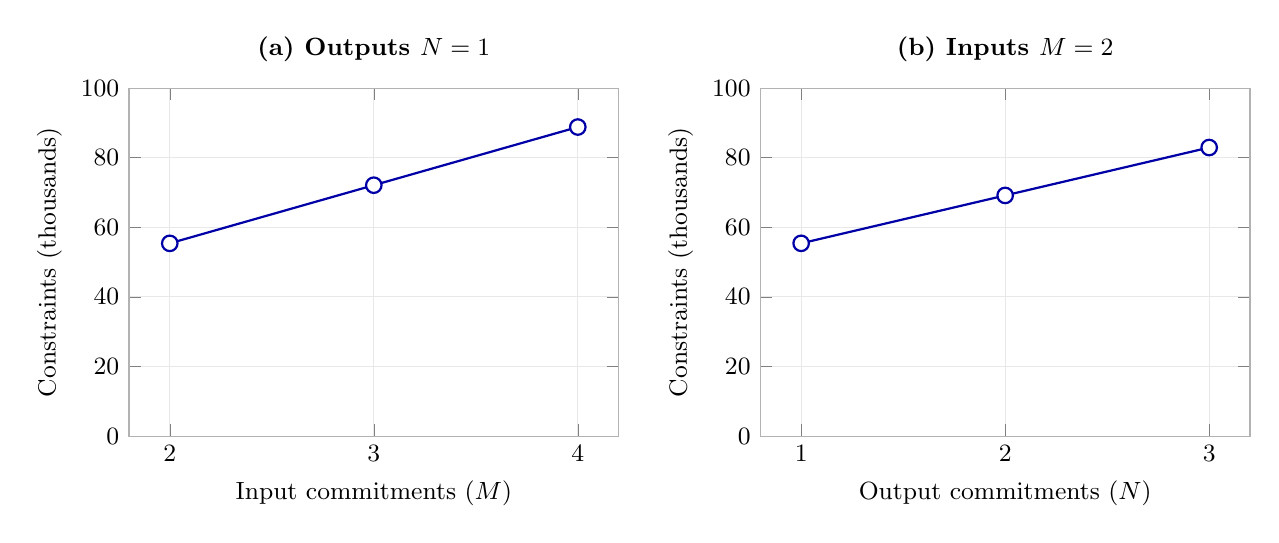
\begin{tikzpicture}
\begin{groupplot}[group style={group size=2 by 1,horizontal sep=1.8cm},width=7.8cm,height=6.0cm,grid=major,major grid style={gray!18},axis line style={gray!60},tick label style={font=\small},label style={font=\small},title style={font=\small\bfseries},legend style={font=\footnotesize,draw=none},scaled ticks=false]
\nextgroupplot[xlabel={Input commitments ($M$)},ylabel={Constraints (thousands)},title={(a) Outputs $N=1$},xtick={2,3,4},ymin=0,ymax=100,legend style={at={(0.5,-0.27)},anchor=north,legend columns=2}]
\addplot+[color=blue!65!black,mark=*,mark size=2.8pt,mark options={solid,fill=white,draw=blue!65!black},thick] coordinates {(2,55.402) (3,72.116) (4,88.832)};

\nextgroupplot[xlabel={Output commitments ($N$)},ylabel={Constraints (thousands)},title={(b) Inputs $M=2$},xtick={1,2,3},ymin=0,ymax=100,legend style={at={(0.5,-0.27)},anchor=north,legend columns=2}]
\addplot+[color=blue!65!black,mark=*,mark size=2.8pt,mark options={solid,fill=white,draw=blue!65!black},thick] coordinates {(1,55.402) (2,69.172) (3,82.944)};

\end{groupplot}
\end{tikzpicture}
\end{document}
